
\begin{document}\documentclass[12pt]{article}

\usepackage{graphicx}
\usepackage{subcaption}
\usepackage{hyperref}

\title{TripEase - Team Benconzaham}
\author{
	Benjamin Karstad
	\texttt{- 101092172}
	\and
	Conor MacQuarrie
	\texttt{- 100824788}
	\and
	Zacharaia Maurice
	\texttt{- 101116412}
	\and
	Graham Shannon
	\texttt{- 100970902}
}


\maketitle
	\pagebreak
	\section*{Architectural Description}
	The intent of TripEase is, above all else, to provide a simple way to keep track of the inanities of vacationing.
	As a team, we broke this problem down into what we thought to be the three most important,
	yet tedious aspects of planning and executing a successful vacation:
	\begin{itemize}
		\item Packing a suitcase
		\item Organizing your time
		\item Managing spending
	\end{itemize}
	Our app's overall architecture was based around these three tasks.
	One of the main themes we chose as a pillar was simpicity and easy of use.
	Keeping the app divided into four tabs (one additional tab for settings and other corner cases) accomplished this.

	The second pillar we chose was on- and offline capability for all primary features.
	Firebase was our chosen storage medium, and it has allowed seamless cloud integration from day one.

	The MVC architecture was a perfect choice for this application, as it mainly displays information statically,
	and allows the user to interactively update.
	Without any external systems other than the firebase cloudstore, the app only needs allow the user to interact,
	then update the server when needed.
	If we were to implement any real-time features, such as a flight status tracker,
	then the observer pattern would provide beneficial aspects;
	as it stands, though, there are no features that would have value added from such an implementation.

	Over-all, the goal of TripEase is to remove the stress of mundane vacationing tasks,
	allowing users to fully take advantage of the time they have to themselves;
	or, in the case of working travellers, limit any external sourced of stress and uncertainty
	so that they may be as productive as possible.

	With this goal in mind, making TripEase as intuitive and user friendly as possible,
	without any extraneous features that could distract from its mission statement is crucial.
	Limiting the functionality to these core features,
	instead of providing a cluttered, "feature rich experience" accomplishes this.

	\pagebreak
	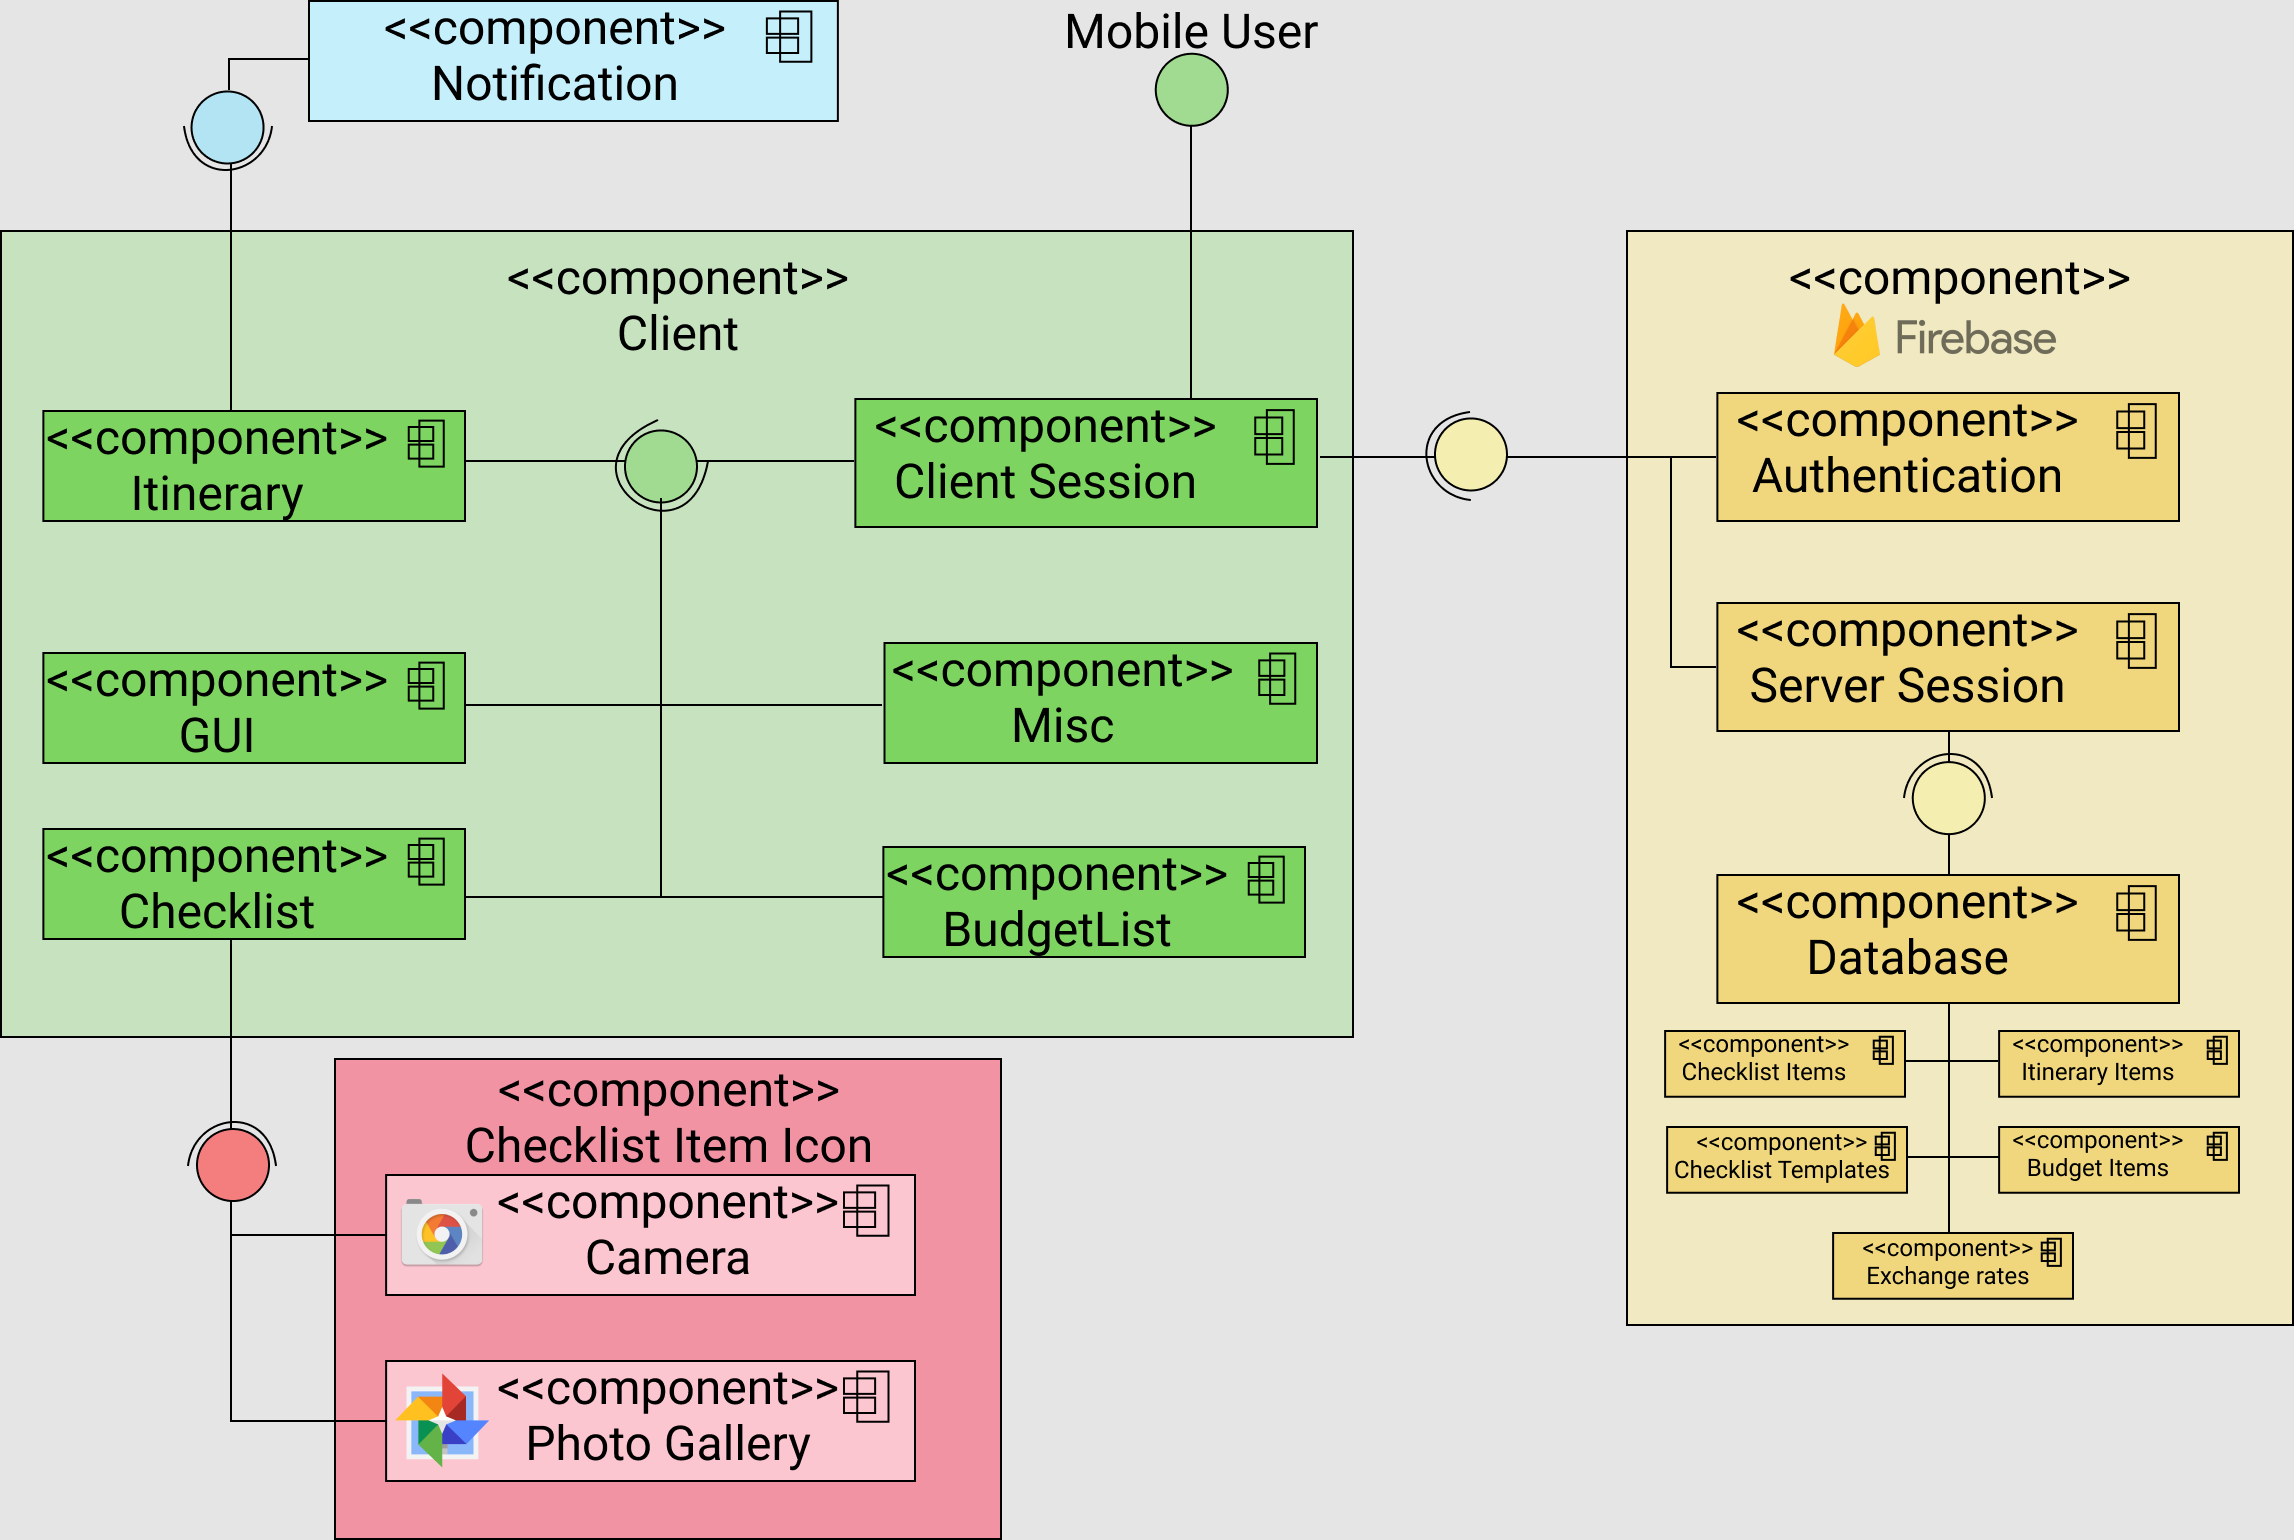
\includegraphics[angle=270,scale=0.4]{Trip-Ease Component Diagram.png}
	\linebreak
	\href{https://www.figma.com/file/VlRhkIKiCqkBc3qPGubwtc/Trip-Ease-Component-Diagram}{Figma Link}
	\pagebreak
	\section*{System Design}

	The design patterns we chose to implement when creating the application was actually more of a mashup than a singular approach. We chose to use a singleton approach
	for our different views as we had concluded that multiple instances of the same view/object occuring would be unnecessary. An example of this would be the way we redirected
	the User Interface. Instead of generating a new view for the user to use as they use the application, we would simply return the already constructed view from earlier.
	This meant that there was less work to be done in the background as the user navigated the application. Since we chose to go with a bottom bar form of navigation-
	this gave us the situation where the clients/users would have a well known access point for everything they need.

	Within the views themselves we decided to go with a more composite approach, following implementation of a template method. Wherein the users created lists/objects would instead of being treated as
	individual elements would be treated instead as a list iteself. The primary reason for this approach, was to allow us the opportunity of having a community based approach to templating.
	A secondary reason for this was that the objects themselves within the lists, would be better treated identically than individually since they are to be able to be maintained,
	deleted, or created- it is best to compound them into the same classification. This would allow us to better manipulate the elements of the list in a more streamlined approach,
	and have it more maintainable for future features to be added and or object types. The reason for the approach of templating the views, in terms of creating a skeleton that the user can
	fill with the parts of their chosing, was to make the process much more transferrable between devices and users themselves. The idea behind having the structure of each of the views
	be a template in design, was for future features. The main one being, users ability to upload their templates- and others being able to download said templates. The reason for this was
	so that a community could potentially develop and users of the application could use each others templates for things such as; packing lists, budgetting, and or iteneraries/scheduling.\\
	\\

	In our app, we minimize coupling and accommodate changing requirements by using fragments and having separate data segments between them.
	The data for any given fragment is stored within itself, and on the database.
	The Checklist fragment has its list items all stored in its own code, the Itinerary fragment has its tasks stored within its section, and the Budget fragment has its own data stored within itself as well.\\


	By using fragments, we can easily accommodate a new addition to the program, or even the removal of another feature from the program if it is no longer deemed necessary.
	To do so, we would simply delete all calls to the fragment and then delete the fragment itself.
	To add a new feature/tab to the program, we would add a new fragment and name it according to the new feature and purpose , and create a route to the fragment through our navigation bar.\\


	In the future if we were to get enough additional features to merit enough additional fragments, we could take an encapsulated approach to categorizing our fragments so that we can separate them by main focus.


	\pagebreak
	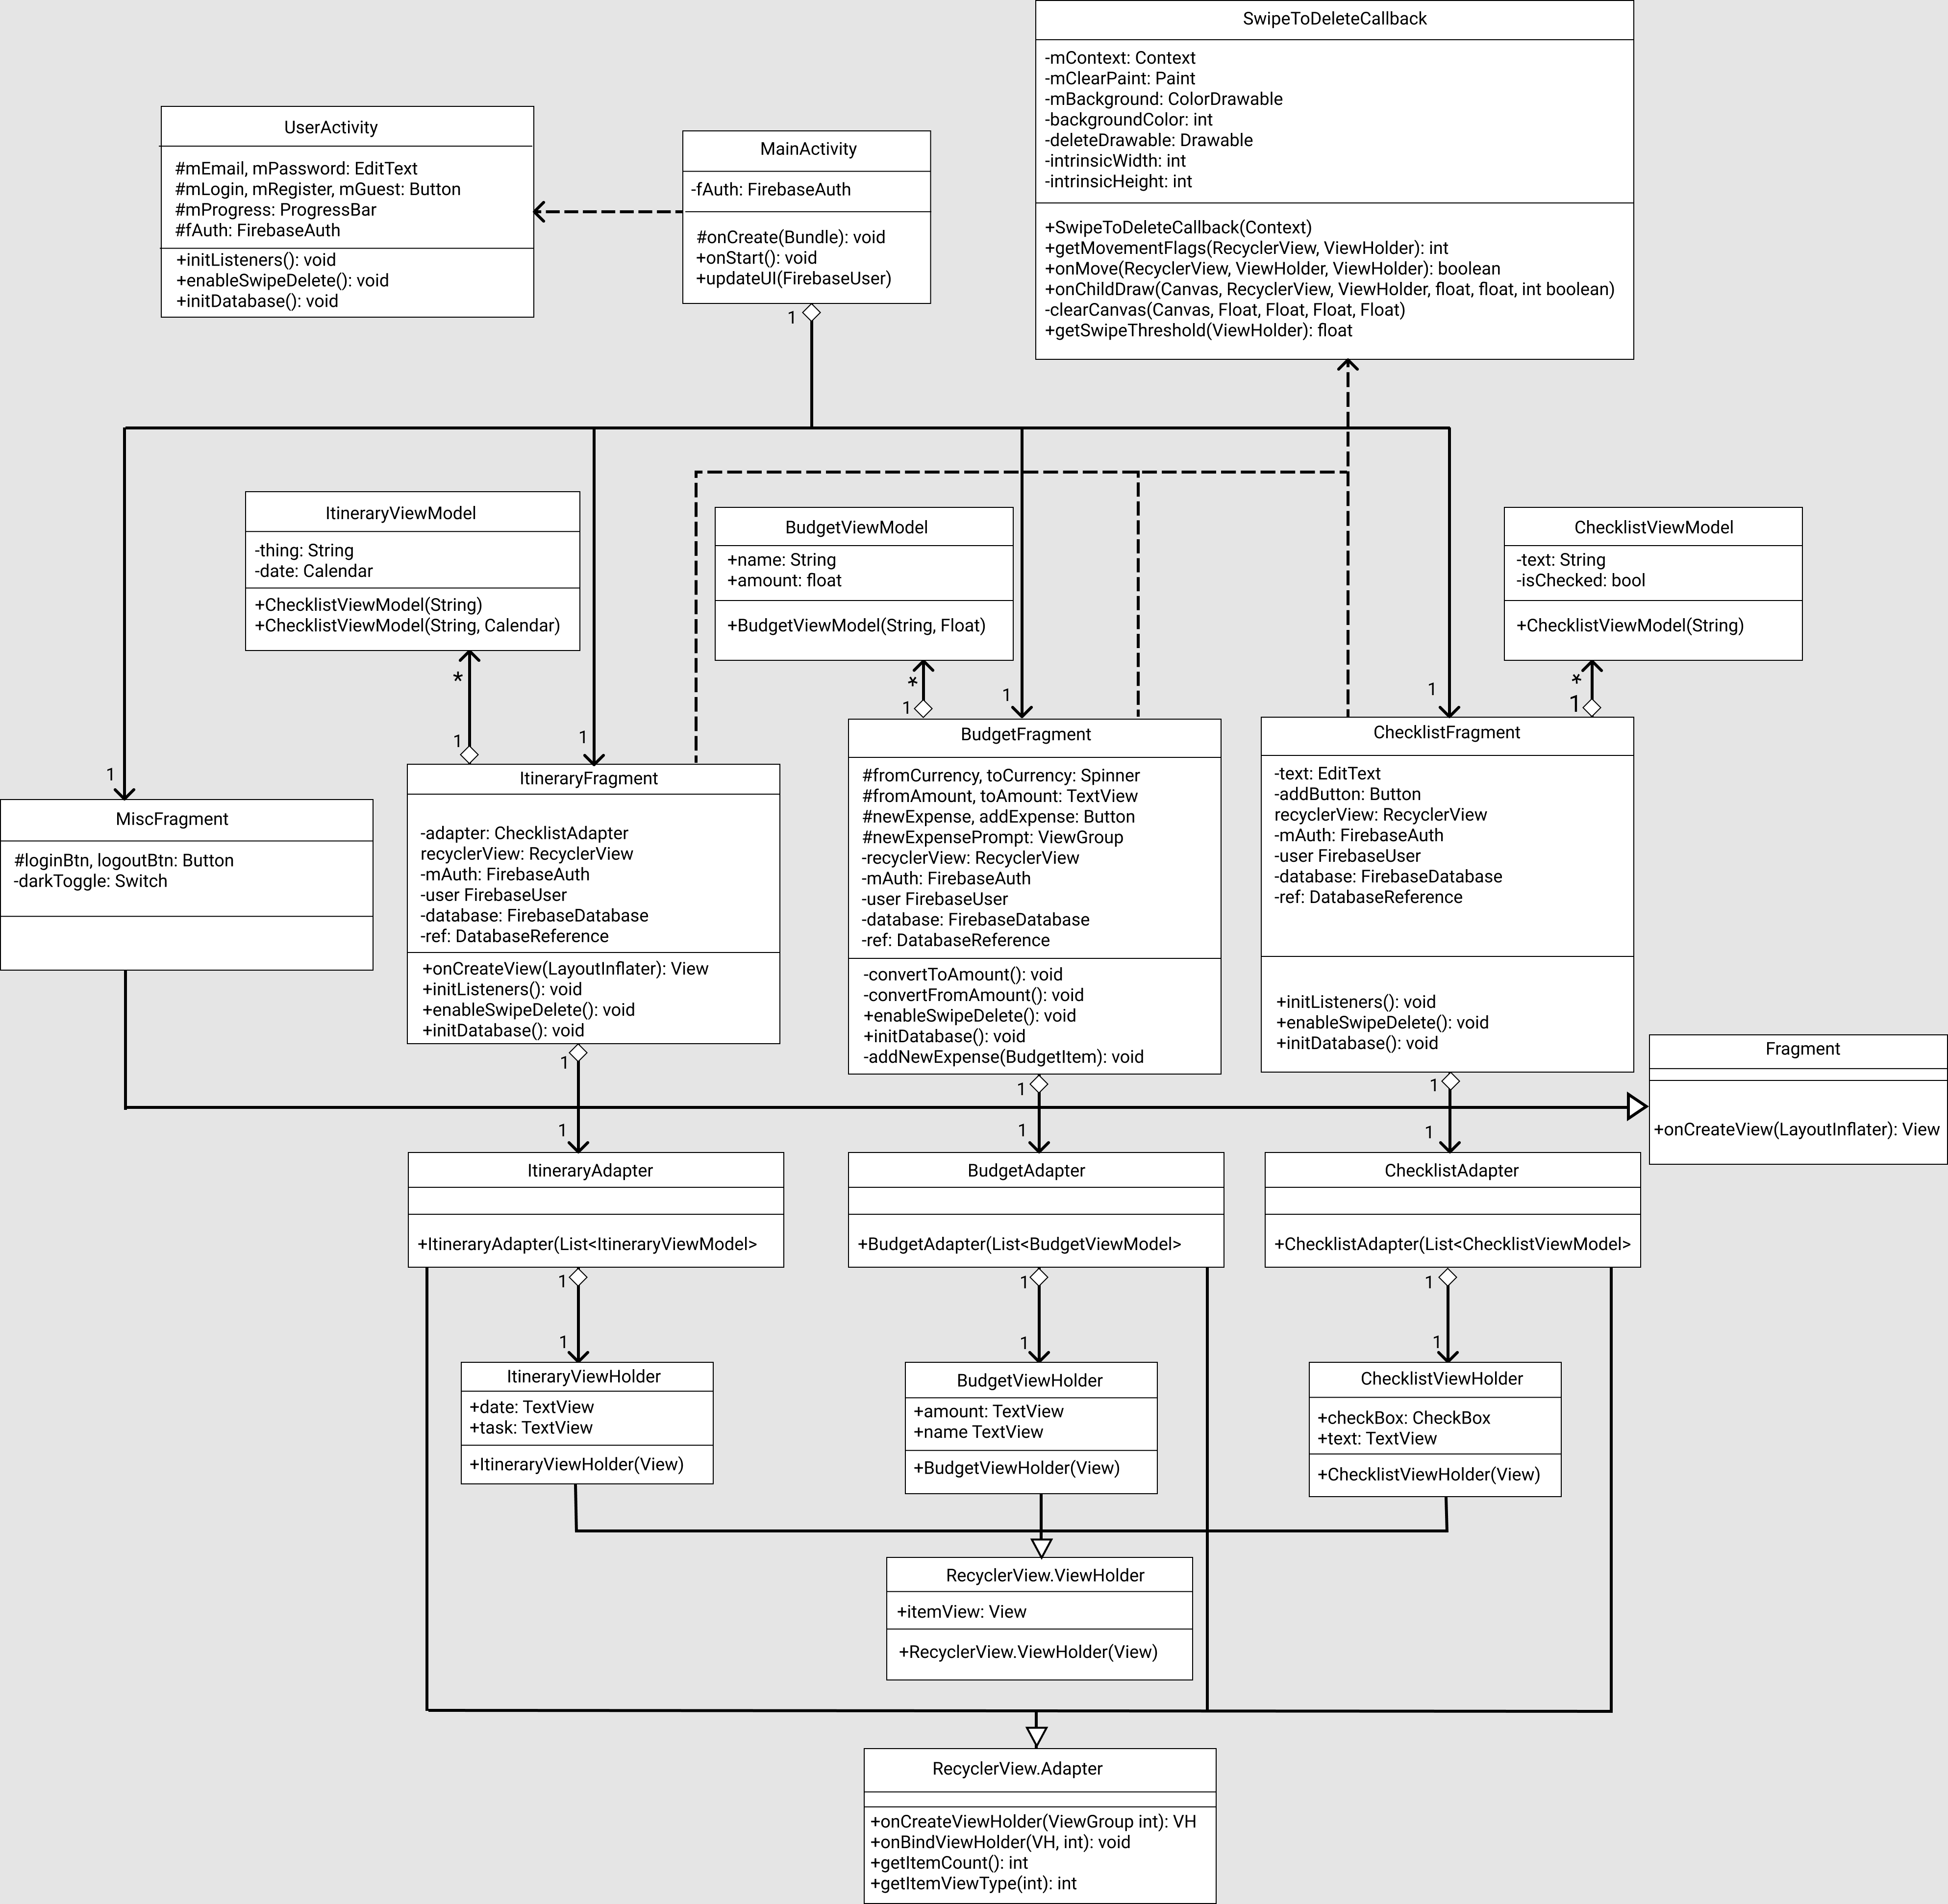
\includegraphics[angle=270,scale=0.2]{Trip-Ease Class Diagram.png}
	\linebreak
	\href{https://www.figma.com/file/TNWldp7eknAI9QecDTNVad/Trip-Ease-Class-Diagram}{Figma Link}
	\pagebreak
	\section*{Task Breakdown}
	We distributed tasks based on which main parts of the program someone would work on, and with four members it was quite simple for us:
	\begin{itemize}
		\item Login\&Registration as well as the initial firebase setup was done by Graham
		\item Checklist fragment was done by Conor
		\item Itinerary fragment was done by Zacharia
		\item Budget fragment was done by Benjamin.
	\end{itemize}
	By splitting the app into four main parts, it allowed each of us to work independently on our own sections and regroup by pushing to the GitHub repository and catching each other up quickly on what was done.
	From this point, we could test each other's work and decide as a group what everyone should work on for the next week or two.
\end{document}
